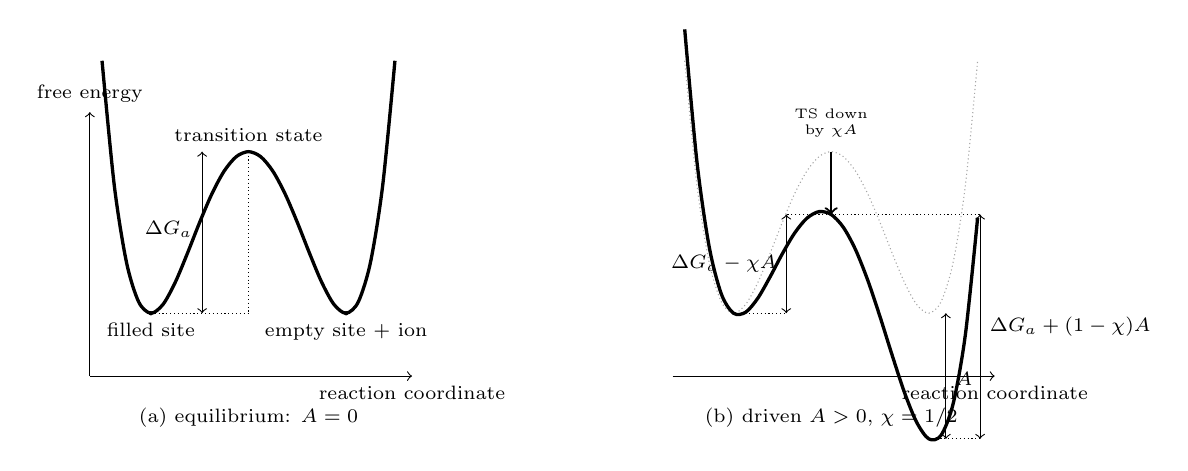
\begin{tikzpicture}[x=0.62cm,y=2.28cm,lab/.style={font=\scriptsize,align=center},tiny/.style={font=\tiny,align=center}]
\draw[->] (-0.25,-0.25)--(6.35,-0.25) node[below,font=\scriptsize] {reaction coordinate};
\draw[->] (-0.25,-0.25)--(-0.25,1.22) node[above,font=\scriptsize] {free energy};
\draw[very thick] plot[smooth] coordinates {(0.0000,1.5063) (0.2500,0.8139) (0.5000,0.3848) (0.7500,0.1635) (1.0000,0.1000) (1.2500,0.1494) (1.5000,0.2723) (1.7500,0.4342) (2.0000,0.6062) (2.2500,0.7647) (2.5000,0.8910) (2.7500,0.9721) (3.0000,1.0000) (3.2500,0.9721) (3.5000,0.8910) (3.7500,0.7647) (4.0000,0.6062) (4.2500,0.4342) (4.5000,0.2723) (4.7500,0.1494) (5.0000,0.1000) (5.2500,0.1635) (5.5000,0.3848) (5.7500,0.8139) (6.0000,1.5063)};
\draw[densely dotted] (1,0.10)--(3,0.10);
\draw[densely dotted] (3,1.00)--(3,0.10);
\draw[<->] (2.05,0.10)--(2.05,1.00) node[pos=0.52,left,font=\scriptsize] {$\Delta G_a$};
\fill (1,0.10) circle (0.8pt) node[below,font=\scriptsize] {filled site};
\fill (5,0.10) circle (0.8pt) node[below,font=\scriptsize] {empty site + ion};
\node[above,font=\scriptsize] at (3,1.00) {transition state};
\node[lab] at (3,-0.48) {(a) equilibrium: $A=0$};
\begin{scope}[xshift=7.40cm]
\draw[->] (-0.25,-0.25)--(6.35,-0.25) node[below,font=\scriptsize] {reaction coordinate};
\draw[black!35,densely dotted] plot[smooth] coordinates {(0.0000,1.5063) (0.2500,0.8139) (0.5000,0.3848) (0.7500,0.1635) (1.0000,0.1000) (1.2500,0.1494) (1.5000,0.2723) (1.7500,0.4342) (2.0000,0.6062) (2.2500,0.7647) (2.5000,0.8910) (2.7500,0.9721) (3.0000,1.0000) (3.2500,0.9721) (3.5000,0.8910) (3.7500,0.7647) (4.0000,0.6062) (4.2500,0.4342) (4.5000,0.2723) (4.7500,0.1494) (5.0000,0.1000) (5.2500,0.1635) (5.5000,0.3848) (5.7500,0.8139) (6.0000,1.5063)};
\draw[very thick] plot[smooth] coordinates {(0.0000,1.6813) (0.2500,0.9451) (0.5000,0.4723) (0.7500,0.2073) (1.0000,0.1000) (1.2500,0.1057) (1.5000,0.1848) (1.7500,0.3030) (2.0000,0.4312) (2.2500,0.5459) (2.5000,0.6285) (2.7500,0.6658) (3.0000,0.6500) (3.2500,0.5783) (3.5000,0.4535) (3.7500,0.2834) (4.0000,0.0813) (4.2500,-0.1345) (4.5000,-0.3402) (4.7500,-0.5068) (5.0000,-0.6000) (5.2500,-0.5802) (5.5000,-0.4027) (5.7500,-0.0174) (6.0000,0.6313)};
\draw[->,thick] (3.00,1.00)--(3.00,0.6500);
\node[tiny] at (3.0,1.16) {TS down\\by $\chi A$};
\draw[densely dotted] (1,0.1000)--(2.08,0.1000);
\draw[densely dotted] (3,0.6500)--(2.08,0.6500);
\draw[<->] (2.08,0.1000)--(2.08,0.6500) node[pos=0.50,left,font=\scriptsize] {$\Delta G_a-\chi A$};
\draw[densely dotted] (5,-0.6000)--(6.05,-0.6000);
\draw[densely dotted] (3,0.6500)--(6.05,0.6500);
\draw[<->] (6.05,-0.6000)--(6.05,0.6500) node[pos=0.50,right,font=\scriptsize] {$\Delta G_a+(1-\chi)A$};
\draw[<->] (5.35,0.1000)--(5.35,-0.6000) node[pos=0.52,right,font=\scriptsize] {$A$};
\node[lab] at (3,-0.48) {(b) driven $A>0$, $\chi=1/2$};
\end{scope}
\end{tikzpicture}
\caption{Eyring 활성화 장벽 개선안. (a) 평형에서는 두 골짜기 높이가 같고 장벽은 $\Delta G_a$ 이다. (b) 구동력 $\mathcal A_j$ 를 주면 도착 골짜기가 낮아지고 전이상태가 반응좌표 분할계수 $\chi$ 만큼 내려가 정방향 장벽은 $\Delta G_a-\chi\mathcal A_j$, 역방향 장벽은 $\Delta G_a+(1-\chi)\mathcal A_j$ 가 된다(식~\eqref{eq:bv}, detailed balance 식~\eqref{eq:db}). 곡선 좌표는 이중우물 quartic 과 선형 tilt 를 Python 으로 수치 평가한 장벽 개형이다.}
\label{fig:barrier}
